\documentclass[11pt]{article}

\usepackage[margin=1in]{geometry}
\usepackage{amsmath,amssymb,amsthm,mathtools}
\usepackage{booktabs}
\usepackage{microtype}
\usepackage{enumitem}
\usepackage{xcolor}
\usepackage{pgfplots}
\pgfplotsset{compat=1.18}
\usepackage{algorithm}
\usepackage{algpseudocode}
\usepackage[hidelinks]{hyperref}

\newtheorem{theorem}{Theorem}
\newtheorem{proposition}[theorem]{Proposition}
\newtheorem{lemma}[theorem]{Lemma}
\newtheorem{corollary}[theorem]{Corollary}
\theoremstyle{definition}
\newtheorem{definition}{Definition}
\newtheorem{assumption}{Assumption}
\renewcommand{\theassumption}{A\arabic{assumption}}
\theoremstyle{remark}
\newtheorem{remark}{Remark}
\newtheorem{example}{Example}

\newcommand{\E}{\mathbb{E}}
\newcommand{\Lucky}{\textup{``Lucky!''}}
\DeclareMathOperator*{\argmin}{arg\,min}

\title{Optimal Play in \emph{Cookie Clicker}:\\[2pt]
\large Purchase Order, Golden-Cookie Banking, Heavenly-Chip Allocation,\\ and Ascension Timing as an Optimal Stopping Problem}
\author{Claude (Anthropic)\\[2pt] \small Prepared for the Cookie~Monster+ project}
\date{October 25, 2026}

\begin{document}
\maketitle

\begin{abstract}
We model the idle game \emph{Cookie Clicker} as a continuous-time growth process with discrete purchases and
periodic resets (``ascensions'') that trade the current run for a permanent production multiplier. Within
explicit models we prove four results. (i)~A pairwise exchange criterion orders purchases by
$p/c + p/\Delta$, and the community ``payback period'' heuristic implements it exactly whenever no candidate is
affordable. (ii)~Holding cookies for the \Lucky{} golden cookie beats buying an item exactly when the item's
payback time, measured on its expected income gain with clicks and golden-cookie effects included, exceeds
$1/(0.15\,g\,\lambda_L)$, about two hours at base golden-cookie frequency.
(iii)~Heavenly chips spent on multiplicative upgrades are allocated optimally by sorting on
$(1-1/m)/p$, a Smith-type ratio rule. (iv)~In the late game, a telescoping lower bound on a Bellman equation yields
a closed-form optimal ascension schedule: each run should multiply all-time cookies by the root $v^\star$ of
$\tfrac{\beta}{3}(1-\tfrac1v) = (1-v^{-\gamma/3})/\gamma$, $\gamma = 3/\beta - 1$, where $\beta$ is the run's growth
exponent. This corrects the marginal value theorem by up to a factor of six. Because the closed form breaks down
early in the game, we give an exact dynamic program over future ascensions that includes heavenly upgrades. In a
simulator built from the game's own building formulas, the stopping rule and the planner reach on average $98.6\%$
and $97.6\%$ of the best outcome in hindsight in late-game scenarios, against $92\%$ for the best fixed rule tuned
per scenario. From a fresh start the planner beats every fixed rule tested by $56\%$ after 30 days. All policies
are implemented in the Cookie~Monster+ mod.
\end{abstract}

\section{Introduction}

\emph{Cookie Clicker} (Orteil, 2013--) is an incremental game. Cookies are produced by clicking and by
buildings whose prices grow geometrically (each copy costs $1.15$ times the previous one); upgrades multiply
production; randomly appearing \emph{golden cookies} grant temporary bonuses; and the player may at any time
\emph{ascend}, abandoning the current run in exchange for \emph{prestige}, a permanent production multiplier
that grows like the cube root of all cookies ever baked. Prestige also yields \emph{heavenly chips}, a currency
for permanent upgrades.

Four decisions recur throughout play: what to buy next, whether to keep cookies in the bank for golden-cookie
rewards, how to spend heavenly chips, and when to ascend. This paper formalises each one, proves optimality
results under stated assumptions, and validates the resulting policies numerically.

\paragraph{Contributions.}
\begin{enumerate}[leftmargin=*,itemsep=2pt]
\item An exchange criterion for purchase order (Theorem~\ref{thm:exchange}), showing that the widely used
``payback period'' ranks purchases optimally whenever nothing is affordable (Corollary~\ref{cor:pp}).
\item A marginal-return rule for holding a \Lucky{} bank (Proposition~\ref{prop:bank}) and a closed form for the
mean golden-cookie interval (Lemma~\ref{lem:interval}).
\item An optimal ratio rule $(1-1/m)/p$ for spending heavenly chips on multiplicative upgrades
(Theorem~\ref{thm:smith}).
\item A time-rescaling lemma (Lemma~\ref{lem:rescale}) that reduces ascension timing to an optimal stopping
problem, a tight lower bound giving the late-game optimum in closed form (Theorem~\ref{thm:lower}), a proof that
early resets are useless when prestige barely affects speed (Proposition~\ref{prop:noprestige}), and an exact
dynamic program for the general case (Proposition~\ref{prop:dp}).
\item Rules for the rest of the game (Section~\ref{sec:rest}): the value of an achievement through milk and, under
time rescaling, in seconds of play (Proposition~\ref{prop:worth}); Godzamok round trips, whose buff grows without
limit when buildings are sold and bought back every frame (Proposition~\ref{prop:godzamok}); the wrinkler factor
$W(n) = 1 - s + s n r$; why wrath cookies beat golden ones under automation, and why calm wins once clicks dominate
(Propositions~\ref{prop:wrath} and~\ref{prop:calm}); and rules for popping wrinklers, the Grimoire (cast at full
magic), the Pantheon, Garden breeding (Lemma~\ref{lem:checkerboard}), Stock Market loans, the dragon, seasons, sugar
lumps, permanent slots and the Born again challenge run.
\item Numerical validation on a simulator using the game's building curves (Section~\ref{sec:numerics}).
\end{enumerate}

\paragraph{Scope.} ``Optimal'' always means optimal \emph{within the stated model}. The proofs are exact under
their assumptions; how well the assumptions fit the real game is tested numerically, not proved. The
policies are implemented in Cookie~Monster+, a fork of the Cookie Monster mod
(Section~\ref{sec:implementation}).

\section{Model}\label{sec:model}

\subsection{Mechanics used}
A run starts with no buildings. Building $k$ with $n$ copies costs $p_k(n) = p_k(0)\,1.15^{\,n}$. Let $A$ be the
number of cookies baked in all previous runs and $C$ the number baked in the current one. Ascending converts the
run into prestige
\begin{equation}\label{eq:prestige}
P(A+C) = \bigl((A+C)/10^{12}\bigr)^{1/3},
\end{equation}
and every prestige level adds $h$ percent to production, where the \emph{prestige power} $h$ becomes $1$ once the
player owns the heavenly upgrade \emph{Legacy} (one chip) and buys five cheap store upgrades
(\emph{Heavenly chip secret} through \emph{Heavenly key}, worth $5\%+20\%+25\%+25\%+25\%$). The production
multiplier of a run that starts at prestige $P$ is therefore
\begin{equation}\label{eq:multiplier}
M(P) = 1 + 0.01\,h\,\lfloor P \rfloor .
\end{equation}
Over the whole game the player receives $\lfloor P\rfloor$ heavenly chips, spent on permanent heavenly upgrades.
Each heavenly upgrade has a price in chips and a set of parent upgrades, all of which must be owned first.

\subsection{Notation}
\begin{center}
\begin{tabular}{@{}ll@{}}
\toprule
Symbol & Meaning \\
\midrule
$c$ & income rate (cookies per second) \\
$b$ & cookies in the bank \\
$p_i,\ \Delta_i$ & price of purchase $i$ and the income it adds \\
$A,\ C$ & cookies baked before the current run, and in it \\
$P$, $h$ & prestige \eqref{eq:prestige}, prestige power \\
$S$ & speed of a run: the factor by which permanent bonuses multiply all income \\
$F(x)$ & run curve: cookies baked after $x$ units of speed-one time \\
$\beta$ & local growth exponent of a run, $\beta = c\,T/C$ \\
$\tau$ & time lost per ascension \\
\bottomrule
\end{tabular}
\end{center}

\subsection{Assumptions}
\begin{assumption}\label{as:piecewise}
Between purchases the income rate is constant, and purchases are instantaneous.
\end{assumption}
\begin{assumption}\label{as:additive}
The income added by a purchase does not depend on the order in which a given pair of purchases is made.
\end{assumption}
\begin{assumption}\label{as:speed}
Permanent bonuses multiply every income source (buildings, clicks, golden-cookie rewards) by the same factor $S$.
\end{assumption}
\begin{assumption}\label{as:scalefree}
Purchase decisions depend on the bank and holdings only through comparisons that are invariant under multiplying
all incomes by a constant.
\end{assumption}
\begin{assumption}\label{as:power}
(Section~\ref{sec:late} only.) The run curve is a power law, $F(x) = \alpha x^{\beta}$ with $\beta > 1$.
\end{assumption}

\section{What to buy next}\label{sec:purchase}

\begin{theorem}[Pairwise exchange]\label{thm:exchange}
Assume \ref{as:piecewise}--\ref{as:additive}. Two purchases $A$ and $B$ are to be made consecutively, starting
from a bank $b \le \min(p_A, p_B)$ and income $c$. Buying $A$ first completes both purchases no later than
buying $B$ first if and only if
\begin{equation}\label{eq:index}
E_A \le E_B, \qquad E_i \coloneqq \frac{p_i}{c} + \frac{p_i}{\Delta_i}.
\end{equation}
Both orders end in the same state.
\end{theorem}

\begin{proof}
With $A$ first, the bank reaches $p_A$ after $(p_A - b)/c$ seconds and is then empty, so $B$ follows after a
further $p_B/(c+\Delta_A)$ seconds:
\[
T_{AB} = \frac{p_A - b}{c} + \frac{p_B}{c + \Delta_A}, \qquad
T_{BA} = \frac{p_B - b}{c} + \frac{p_A}{c + \Delta_B}.
\]
The bank $b$ cancels in $T_{AB} - T_{BA}$, and
\[
T_{AB} \le T_{BA}
\iff p_A\Bigl(\frac1c - \frac{1}{c+\Delta_B}\Bigr) \le p_B\Bigl(\frac1c - \frac{1}{c+\Delta_A}\Bigr)
\iff \frac{p_A\Delta_B}{c+\Delta_B} \le \frac{p_B\Delta_A}{c+\Delta_A}.
\]
Multiplying by $(c+\Delta_A)(c+\Delta_B)/(c\,\Delta_A\Delta_B) > 0$ gives
$p_A/\Delta_A + p_A/c \le p_B/\Delta_B + p_B/c$. After both purchases the holdings, the empty bank and the income
$c+\Delta_A+\Delta_B$ (by \ref{as:additive}) coincide.
\end{proof}

\begin{remark}\label{rem:local}
Because both orders end in the same state, any objective of the form ``reach a given state as early as
possible'' prefers the order with the smaller index. Buying, at each decision, the candidate with the smallest
$E_i$ at the current income is therefore \emph{locally optimal}: no swap of two consecutive purchases improves it.
A single global sort is impossible, because $E_i$ depends on $c$, which grows.
\end{remark}

\begin{corollary}[Payback period]\label{cor:pp}
Cookie Monster ranks purchases by the payback period
$\mathrm{PP}_i = \max(p_i - b, 0)/c + p_i/\Delta_i$. When no candidate is affordable, $\mathrm{PP}_i = E_i - b/c$,
so the payback period and the exchange index induce the same ranking.
\end{corollary}

\begin{proposition}[Affordable pairs]\label{prop:affordable}
If $\max(p_A,p_B) \le b < p_A + p_B$, buying $A$ first is better if and only if $\Delta_A > \Delta_B$.
\end{proposition}

\begin{proof}
Buying $A$ immediately leaves $b - p_A < p_B$, and the remaining $p_A + p_B - b$ cookies arrive at rate
$c+\Delta_A$: $T_{AB} = (p_A+p_B-b)/(c+\Delta_A)$. The expression for $T_{BA}$ is symmetric, and the
numerators agree.
\end{proof}

With a large bank the exchange index is therefore not exact. Section~\ref{sec:numerics} shows the effect is small:
over nine scenarios, replacing the payback period by the bank-independent index, or adding a look-ahead to tier
upgrades, changes the time to reach a target by at most $0.35\%$ in continuous play and $1.7\%$ when purchases are
made only once an hour.

\section{Golden cookies and the bank}\label{sec:golden}

\subsection{When to hold a \Lucky{} bank}
A \Lucky{} golden cookie pays $\min(0.15\,b,\ 900\,c)\,g + 13$ cookies, where $g$ collects golden-cookie gain
multipliers. Below the cap ($b < 6000\,c$) the reward is linear in the bank.

\begin{proposition}[Marginal value of banked cookies]\label{prop:bank}
Let \Lucky{} events occur at rate $\lambda_L$ and let $b < 6000\,c$. A marginal banked cookie earns
$0.15\,g\,\lambda_L$ cookies per second in expectation, while spending it on item $i$ earns $\bar\Delta_i/p_i$,
where $\bar\Delta_i$ is the expected increase in total income the item brings (Definition~\ref{def:auto}).
Spending is better if and only if
\[
\frac{p_i}{\bar\Delta_i} \;<\; \theta \coloneqq \frac{1}{0.15\,g\,\lambda_L}.
\]
\end{proposition}

\begin{proof}
Below the cap, each \Lucky{} event pays $0.15\,g$ per banked cookie, and these events arrive at rate
$\lambda_L$. By linearity of expectation the banked cookie returns $0.15\,g\,\lambda_L$ per second. A cookie spent
on item $i$ returns $\bar\Delta_i/p_i$ per second. Comparing the two marginal returns gives the claim.
\end{proof}

Without golden cookies or clicking, $\bar\Delta_i$ is the CpS gain $\Delta_i$. With both automated, using
$\Delta_i$ instead undervalues every purchase: with both frequency upgrades and a fast auto-clicker, golden cookies
and clicks multiply a CpS gain about eightfold (Example~\ref{ex:theta}), so purchases whose payback lies between
$\theta$ and several times $\theta$ would be held although buying them is better.

The rate is $\lambda_L = \pi_L/\E[I]$, where $\pi_L \approx 0.42$ is the probability that a golden cookie is
\Lucky{} and $I$ is the interval between golden cookies.

\begin{lemma}[Golden-cookie interval]\label{lem:interval}
Golden cookies spawn between $t_{\min}$ and $t_{\max}$. In each frame of the window the spawn probability is
$((t-t_{\min})/W)^5$, where $t$ is the current frame and the window lasts $W$ frames. Writing
$I = t_{\min} + x\,(t_{\max}-t_{\min})$,
\[
\E[x] \approx \Gamma\!\left(\tfrac76\right) \left(\frac{6}{W}\right)^{1/6}.
\]
\end{lemma}

\begin{proof}
The probability of surviving to fraction $x$ of the window is
\[
\prod_{k \le xW} \bigl(1 - (k/W)^5\bigr) \approx \exp\Bigl(-W \int_0^x u^5\,du\Bigr) = \exp(-W x^6/6).
\]
Hence, using $\int_0^\infty e^{-a x^n}dx = a^{-1/n}\,\Gamma(1+1/n)$,
\[
\E[x] = \int_0^1 e^{-Wx^6/6}\,dx \approx \int_0^\infty e^{-Wx^6/6}\,dx = \Bigl(\frac{6}{W}\Bigr)^{1/6}\Gamma\!\left(\tfrac76\right).
\qedhere
\]
\end{proof}

\begin{example}\label{ex:theta}
At base frequency ($t_{\min} = 5$\,min, $t_{\max} = 15$\,min, $30$ frames per second, $W = 18000$),
$\E[x] \approx 0.244$ and $\E[I] \approx 447$\,s. With both frequency-doubling upgrades $W = 4500$ and
$\E[x] \approx 0.308$. Taking $\pi_L = 0.42$ and $g = 1$ gives $\theta \approx 7.1\times10^3$\,s, about two hours,
at base frequency and $\theta \approx 1.9\times10^3$\,s with both upgrades ($\E[I] \approx 121$\,s). In the second
case, with building specials on types averaging $\bar n = 60$ (Definition~\ref{def:auto}), $1 + \sigma_c \approx 4.5$
and $1 + \sigma_k \approx 6.1$. With three mouse upgrades ($+1\%$ of CpS per click each) at $r = 20$ clicks per
second, $r\,\delta_i = 0.6\,\Delta_i$, so $\bar\Delta_i \approx 8.2\,\Delta_i$. A purchase is then held only if its
CpS payback $p_i/\Delta_i$ exceeds about $8.2\,\theta \approx 1.6\times10^4$\,s, four and a half hours.
Early in a run payback times are seconds to minutes, so every cookie should be spent. Late in a run payback
times are hours to days, so the \Lucky{} bank should be kept.
\end{example}

\subsection{Values under automation}
Cookie Monster's simulator values upgrades by the CpS they add, so click upgrades and golden-cookie upgrades
show a value of zero. Under automation they have a definite value.
\begin{definition}[Automation values]\label{def:auto}
Let $c$ be CpS and $k$ the income of an auto-clicker at $r$ clicks per second. A purchase adds $\Delta_i$ to $c$
and $r\,\delta_i$ to $k$, where $\delta_i$ is its gain in cookies per click, including click power that is a share
of CpS. If every golden cookie is clicked as it appears, the outcomes and their shares under the game's choice rule
are: Frenzy ($\pi_F \approx 0.42$; production $\times 7$ for $77\,d$\,s), \Lucky{} ($\pi_L \approx 0.42$;
$\min(0.15\,b,\ 900\,c)\,g$), building special ($\pi_B \approx 0.10$; CpS $\times (1 + n/10)$ for $30\,d$\,s, where $n$ is
the count of a random building type with at least ten), Click frenzy ($\pi_C \approx 0.04$; clicks $\times 777$ for
$13\,d$\,s) and cookie storm ($\pi_S \approx 0.0085$; about $105\,d$ drops worth one to seven minutes of CpS each),
with $d = 2$ under \emph{Get lucky}. Per unit of CpS and of click income they add, on average,
\[
\sigma_c = \frac{(462\,\pi_F + 3\bar n\,\pi_B + 25200\,g\,\pi_S)\,d}{\E[I]},\qquad
\sigma_k = \frac{(462\,\pi_F + 3\bar n\,\pi_B + 10088\,\pi_C)\,d}{\E[I]},
\]
where $\bar n$ is the mean count over building types with at least ten; Frenzies and building specials multiply
CpS and so also the click power derived from it. Below the cap \Lucky{} pays a share of the bank, not of
production, so a purchase raises expected income by
\[
\bar\Delta_i = (1 + \sigma_c)\,\Delta_i + (1 + \sigma_k)\,r\,\delta_i.
\]
Golden cookies bring in $G = \sigma_c\,c + \sigma_k\,k + \lambda_L\,g \min(0.15\,b,\ 900\,c)$ in all, so expected
income, which fills the bank, is $c + k + G$. \emph{Lucky day} and \emph{Serendipity}, which double the frequency,
are worth $G$ each; \emph{Get lucky}, which doubles every duration, is worth $\sigma_c\,c + \sigma_k\,k$; and
\emph{Golden goose egg} (+5\% frequency) is worth $0.05\,G$.
\end{definition}
With income and gains measured this way, Theorem~\ref{thm:exchange} and Proposition~\ref{prop:bank} apply
unchanged. Both are computed without the buffs active at the moment, since a Frenzy would otherwise make every
purchase look seven times better for its 77 seconds. The heavenly-upgrade values of Table~\ref{tab:heavenly} use
the simpler shares $\sigma_F = 462\,\pi_F\,d/\E[I]$ and $\sigma = \sigma_F + \pi_L \min(900,\ 0.15\,b/c)\,g/\E[I]$,
which count Frenzies and \Lucky{} only.

\section{Spending heavenly chips}\label{sec:chips}

Chips arrive over the course of the game. Earning the chips between budget levels $B$ and $B+dB$ takes time
$g(B)\,dB/S(B)$. Here $g$ reflects how many cookies each chip costs, which is the same whatever has been bought,
and $S(B)$ is the speed. Buying heavenly upgrade $j$ costs $p_j$ chips and multiplies $S$ by $m_j > 1$; the
prestige factor~\eqref{eq:multiplier} is common to all orders and can be absorbed into $g$.

\begin{theorem}[Ratio rule for multiplicative speed-ups]\label{thm:smith}
Suppose there are no parent constraints and $g$ is constant over the budget range considered. Then the order of
purchases minimising the total time sorts items by
\[
\rho_j = \frac{1 - 1/m_j}{p_j}
\]
in decreasing order. Any order that is not sorted can be strictly improved by swapping an adjacent pair.
\end{theorem}

\begin{proof}
Let $\Pi$ be the product of the multipliers bought before two adjacent items $i$ and $j$. Swapping them leaves
every other term unchanged, because after both items the product is $\Pi m_i m_j$ in either order. Their own
contribution is $g(p_i + p_j/m_i)/(S_0\Pi)$ with $i$ first and $g(p_j + p_i/m_j)/(S_0\Pi)$ with $j$ first, where
$S_0$ is the initial speed. Hence $i$ first is strictly better if and only if
\[
p_i + \frac{p_j}{m_i} < p_j + \frac{p_i}{m_j}
\iff p_i\Bigl(1 - \frac{1}{m_j}\Bigr) < p_j\Bigl(1 - \frac{1}{m_i}\Bigr)
\iff \rho_i > \rho_j .
\]
An unsorted order contains an adjacent inverted pair, and swapping it strictly reduces the total time. There are
finitely many orders, so a sorted order is optimal.
\end{proof}

\begin{remark}\label{rem:chips}
\begin{enumerate}[leftmargin=*,itemsep=2pt,label=(\alph*)]
\item For small effects $1 - 1/m \approx \ln m$, so the rule reduces to log-gain per chip. For large effects the
two differ: \emph{Heralds} can be worth $m = 2$.
\item The rule implies \emph{saving up}. Buying a cheaper, lower-ratio item first delays a higher-ratio one, which
the interchange argument shows is worse. Cookie~Monster+ therefore spends chips along the sorted order and stops
at the first unaffordable item.
\item Parent constraints are handled by treating an upgrade together with its unowned ancestors as a single block
with multiplier $\prod m$ and cost $\sum p$. The interchange argument applies verbatim to adjacent blocks, which is
the idea behind Sidney's decomposition for scheduling with precedence constraints
(Sidney, 1975; see also Lawler, 1978). We restrict blocks to ancestor closures of single upgrades. This is exact
without constraints (Theorem~\ref{thm:smith}; a unit test checks it against brute force on random instances) and a
heuristic in general.
\end{enumerate}
\end{remark}

Table~\ref{tab:heavenly} lists the multipliers used. They follow the in-game descriptions where the effect on
production is direct, and are marked as estimates where the effect works through cheaper or newly unlocked store
upgrades.

\begin{table}[t]
\centering
\small
\begin{tabular}{@{}lrl@{}}
\toprule
Heavenly upgrade & Chips & Production multiplier $m$ \\
\midrule
Heavenly cookies & 3 & $1.10$ \\
Heralds & 100 & $1 + 0.01\cdot\text{heralds}$ (heralds $\le 100$) \\
Heavenly luck & 77 & $1 + 0.05\,\sigma$ \\
Lasting fortune & 777 & $1 + 0.10\,\sigma_F$ \\
Lucky digit & 777 & $1.01\,(1 + 0.01\,\sigma_F)$ \\
Lucky number & 77{,}777 & $1.01\,(1 + 0.01\,\sigma_F)$ \\
Lucky payout & 77{,}777{,}777 & $1.01\,(1 + 0.01\,\sigma_F)$ \\
Kitten angels & 9{,}000 & $1 + 0.1\cdot\text{milk}$ \\
Halo gloves & 55{,}555 & $1 + 0.1\,s_{\mathrm{click}}$ \\
Wrinkly cookies & 6{,}666{,}666 & $1.10$ \\
Distilled essence of redoubled luck & 7{,}777{,}777 & $1 + 0.01\,\sigma$ \\
Sugar baking & $2\times10^{8}$ & $1 + 0.01\min(\text{unspent lumps}, 100)$ \\
Sugar crystal cookies & $10^{9}$ & $1.05$ \\
Divine discount & 99{,}999 & $1.01$ (estimate) \\
Divine sales & 99{,}999 & $1.005$ (estimate) \\
Divine bakeries & 399{,}999 & $1.03$ (estimate) \\
Synergies Vol.~I / Vol.~II & 222{,}222 / 2{,}222{,}222 & $1.05$ each (estimate) \\
Cookie boxes, four early / three late & 25 / $3.3\times10^{11}$ & $1.02$ each (estimate) \\
Persistent memory & 500 & $1.01$ (estimate) \\
Starter kit / Starter kitchen & 50 / 5{,}000 & $1.005$ each (estimate) \\
\bottomrule
\end{tabular}
\caption{Heavenly upgrades valued by the allocation rule; $s_{\mathrm{click}}$ is the share of income from
clicks. Chips are list prices; parents are added when blocks are formed. Cosmetics, switches, offline production, the dragon, wrinklers, seasons, fortunes and permanent upgrade
slots are bought only as parents of valued upgrades.}
\label{tab:heavenly}
\end{table}

\section{When to ascend}\label{sec:ascension}

\subsection{Time rescaling}

\begin{lemma}[Time rescaling]\label{lem:rescale}
Assume \ref{as:piecewise}, \ref{as:speed} and \ref{as:scalefree}. If a run at speed $1$ bakes $F(x)$ cookies in
time $x$, then the same run at speed $S$ bakes $F(S\,t)$ cookies in time $t$.
\end{lemma}

\begin{proof}
Let $q(t)$ be the holdings and $r(q)$ the base income. At speed $S$ the bank obeys $\dot b = S\,r(q)$ between
purchases, and by \ref{as:scalefree} purchase decisions depend only on $(b,q)$. In the time variable
$\tilde t = S t$ the dynamics are $db/d\tilde t = r(q)$ with the same decision rule, independent of $S$. Hence the
path $(b,q)(\tilde t)$ is the same for every $S$, and the cookies baked, $\int r\,d\tilde t$, equal $F(\tilde t)$.
\end{proof}

Ranking purchases by payback period satisfies \ref{as:scalefree}, since every $\mathrm{PP}_i$ scales by $1/S$.
Golden cookies, whose spawn clock runs in real time, and the \Lucky{} reserve, which scales with $S$, satisfy it
only approximately.

\subsection{Formulation}
Run $k$ starts with all-time cookies $A_k$ and speed $S_k = S(P(A_k))$. If it lasts $T_k$, it bakes
$C_k = F(S_k T_k)$ (Lemma~\ref{lem:rescale}) and $A_{k+1} = A_k + C_k$. The player chooses the run lengths to
minimise the total time $\sum_k (T_k + \tau)$ needed to reach a distant goal $A^\ast$. This is an optimal stopping
problem with Bellman equation
\begin{equation}\label{eq:bellman}
V(A) = \min_{A' > A} \Bigl[\,T(A \to A') + \tau + V(A')\,\Bigr], \qquad V(A^\ast) = 0 .
\end{equation}

\subsection{Late game: a closed form}\label{sec:late}
In the late game $M(P) \approx 0.01\,h\,P$, so $S(P) = \kappa P$. Take $\tau = 0$ and assume~\ref{as:power}. Let
$y = \ln P$. A run whose log-prestige grows by $\Delta$ must bake $C = 10^{12}P^3(e^{3\Delta} - 1)$ cookies, which
at speed $\kappa P$ takes
\begin{equation}\label{eq:runtime}
T(y,\Delta) = \frac{(C/\alpha)^{1/\beta}}{\kappa P} = K\,e^{\gamma y}\,\varphi(\Delta), \qquad
\varphi(\Delta) = (e^{3\Delta}-1)^{1/\beta}, \quad \gamma = \frac{3}{\beta} - 1, \quad
K = \frac{(10^{12}/\alpha)^{1/\beta}}{\kappa}.
\end{equation}
When $\gamma > 0$ ($\beta < 3$), runs get longer as prestige grows; when $\gamma < 0$ they get shorter.

\begin{theorem}[Lower bound and optimal step]\label{thm:lower}
Let $G(\Delta) = (e^{\gamma\Delta}-1)/\gamma$ (with $G(\Delta) = \Delta$ if $\gamma = 0$) and
$w = \inf_{\Delta > 0} K\varphi(\Delta)/G(\Delta)$. Every ascension schedule from $y_0$ to $y^\ast$ satisfies
\[
\sum_k T_k \;\ge\; \frac{w}{\gamma}\bigl(e^{\gamma y^\ast} - e^{\gamma y_0}\bigr)
\qquad \Bigl(\text{resp. } w\,(y^\ast - y_0) \text{ if } \gamma = 0\Bigr),
\]
with equality if and only if every step $\Delta_k$ minimises $\varphi/G$. For $\beta > 1$ a minimiser
$\Delta^\star$ exists.
\end{theorem}

\begin{proof}
For $\gamma \neq 0$, $G(\Delta) > 0$ for $\Delta > 0$, and
$e^{\gamma y}G(\Delta) = (e^{\gamma(y+\Delta)} - e^{\gamma y})/\gamma$. By definition of $w$,
$K\varphi(\Delta) \ge w\,G(\Delta)$ for every $\Delta > 0$. With $y_{k+1} = y_k + \Delta_k$,
\[
\sum_k T_k = \sum_k K e^{\gamma y_k}\varphi(\Delta_k) \ge w \sum_k e^{\gamma y_k} G(\Delta_k)
= \frac{w}{\gamma}\sum_k \bigl(e^{\gamma y_{k+1}} - e^{\gamma y_k}\bigr)
= \frac{w}{\gamma}\bigl(e^{\gamma y^\ast} - e^{\gamma y_0}\bigr),
\]
a telescoping sum. The only inequality used is an equality exactly when $K\varphi(\Delta_k) = wG(\Delta_k)$ for
every $k$. The case $\gamma = 0$ is identical with $G(\Delta) = \Delta$.

For existence: as $\Delta \to 0^+$, $\varphi(\Delta)/G(\Delta) \sim 3^{1/\beta}\Delta^{1/\beta - 1} \to \infty$
because $\beta > 1$. As $\Delta \to \infty$, $\varphi(\Delta) \sim e^{3\Delta/\beta}$ while $G$ grows at most like
$e^{\gamma\Delta}/\gamma$ with $\gamma < 3/\beta$, so the ratio again tends to infinity. A continuous function on
$(0,\infty)$ that tends to infinity at both ends attains its minimum.
\end{proof}

The bound is achieved by repeating the step $\Delta^\star$, up to the rounding of the last step before the goal.
For $\beta \le 1$ the ratio $\varphi/G$ has no interior minimum and resets should be as frequent as overhead
allows. This degenerate case motivates a safeguard in the implementation (Section~\ref{sec:dp}).

\begin{corollary}[Stopping rule]\label{cor:stop}
At an interior minimiser $\varphi'/\varphi = G'/G$. Since the current run's length is proportional to
$\varphi(\Delta)$, the optimal moment to ascend is when the run's marginal log-prestige rate falls to
\[
\frac{d\Delta}{dT} = \frac{1 - e^{-\gamma\Delta}}{\gamma\,T}.
\]
For a run whose cookies grow like $T^\beta$, $\Delta = \tfrac13\ln v$ with $v = (A+C)/A$ and
$d\Delta/dT = \tfrac{\beta}{3}(1 - 1/v)/T$. Ascending is optimal when all-time cookies have grown by the factor
$v^\star$ solving
\begin{equation}\label{eq:vstar}
\frac{\beta}{3}\Bigl(1 - \frac1v\Bigr) = \frac{1 - v^{-\gamma/3}}{\gamma}.
\end{equation}
\end{corollary}

\begin{proof}
$T'(\Delta)/T(\Delta) = \varphi'/\varphi = G'/G$, hence
$d\Delta/dT = G/(G'\,T) = (e^{\gamma\Delta}-1)/(\gamma e^{\gamma\Delta}T)$. With $C \propto T^\beta$ we have
$dv/dT = \beta(v-1)/T$, so $d\Delta/dT = \tfrac{1}{3v}\,dv/dT$. Equating the two expressions gives
\eqref{eq:vstar}.
\end{proof}

\begin{remark}[The marginal value theorem]\label{rem:mvt}
For $\gamma = 0$ ($\beta = 3$) the rule reads $d\Delta/dT = \Delta/T$: ascend when the marginal rate equals the
average rate. This is the marginal value theorem of optimal foraging (Charnov, 1976). Applying it when
$\beta \neq 3$ ignores that later runs get longer or shorter. It solves $\beta(v-1) = v\ln v$ instead of
\eqref{eq:vstar} and errs by a factor of $1.6$ at $\beta = 2$ and $6.5$ at $\beta = 6$ (Table~\ref{tab:vstar}).
\end{remark}

\begin{remark}[Overhead]
With $\tau > 0$ the problem is no longer self-similar. Corollary~\ref{cor:stop} then holds approximately with $T$
replaced by $T+\tau$; the general problem is solved exactly by dynamic programming (Section~\ref{sec:dp}).
\end{remark}

\begin{table}[t]
\centering
\small
\begin{tabular}{@{}rrrrrrr@{}}
\toprule
$\beta$ & $\gamma$ & $v^\star$ (eq.~\ref{eq:vstar}) & prestige $\times$ per run & naive MVT $v$ & brute force & dynamic program \\
\midrule
1.5 & 1.000 & 4.24 & 1.62 & 2.40 & 4.42 & 4.39 \\
2.0 & 0.500 & 7.87 & 1.99 & 4.92 & 7.95 & 7.18 \\
2.5 & 0.200 & 12.03 & 2.29 & 9.31 & 11.49 & 11.50 \\
3.0 & 0.000 & 16.80 & 2.56 & 16.80 & 15.95 & 16.69 \\
4.0 & $-0.250$ & 28.39 & 3.05 & 50.44 & 31.69 & 28.95 \\
6.0 & $-0.500$ & 60.91 & 3.93 & 397.38 & 63.59 & 60.13 \\
\bottomrule
\end{tabular}
\caption{Optimal factor $v^\star$ by which each run multiplies all-time cookies in the late game. ``Brute force''
scans fixed factors to grow prestige a millionfold (the last, partial run causes the scatter). ``Dynamic
program'' is the planner of Section~\ref{sec:dp}, averaged over runs that have baked $0.1$, $0.5$ and $2$ times
the previous all-time cookies.}
\label{tab:vstar}
\end{table}

\begin{figure}[t]
\centering
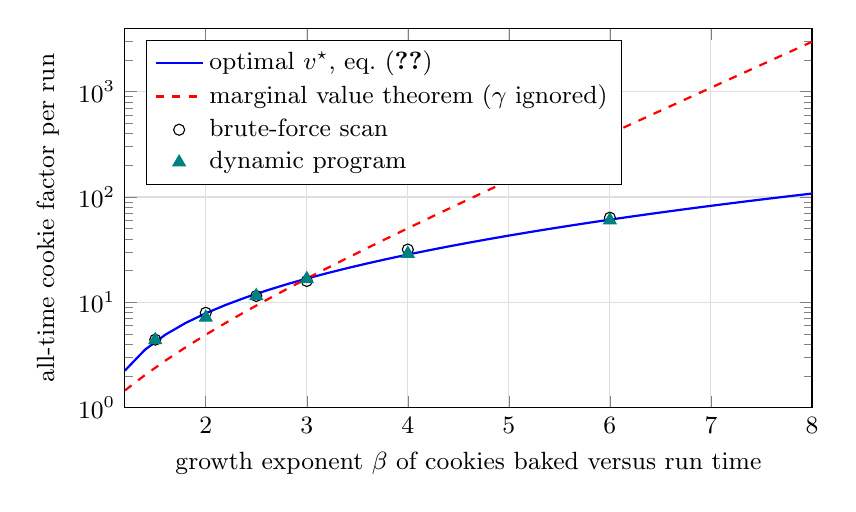
\begin{tikzpicture}
\begin{semilogyaxis}[
  width=0.85\linewidth, height=6.4cm,
  xlabel={growth exponent $\beta$ of cookies baked versus run time},
  ylabel={all-time cookie factor per run},
  xmin=1.2, xmax=8, ymin=1, ymax=4000,
  legend pos=north west, legend cell align=left, grid=major, grid style={gray!25},
  tick label style={font=\small}, label style={font=\small}, legend style={font=\small}]
\addplot[thick, blue] coordinates {(1.2,2.250) (1.4,3.560) (1.6,4.927) (1.8,6.361) (2.0,7.872) (2.2,9.467) (2.4,11.153) (2.6,12.934) (2.8,14.816) (3.0,16.801) (3.2,18.893) (3.4,21.095) (3.6,23.410) (3.8,25.841) (4.0,28.390) (4.2,31.060) (4.4,33.853) (4.6,36.772) (4.8,39.818) (5.0,42.995) (5.2,46.305) (5.4,49.749) (5.6,53.330) (5.8,57.050) (6.0,60.912) (6.2,64.917) (6.4,69.068) (6.6,73.367) (6.8,77.816) (7.0,82.417) (7.2,87.172) (7.4,92.083) (7.6,97.153) (7.8,102.384) (8.0,107.777)};
\addlegendentry{optimal $v^\star$, eq.~\eqref{eq:vstar}}
\addplot[thick, red, dashed] coordinates {(1.2,1.457) (1.4,2.045) (1.6,2.793) (1.8,3.737) (2.0,4.922) (2.2,6.400) (2.4,8.237) (2.6,10.514) (2.8,13.329) (3.0,16.801) (3.2,21.077) (3.4,26.335) (3.6,32.793) (3.8,40.718) (4.0,50.435) (4.2,62.342) (4.4,76.923) (4.6,94.771) (4.8,116.610) (5.0,143.325) (5.2,175.995) (5.4,215.938) (5.6,264.767) (5.8,324.447) (6.0,397.383) (6.2,486.509) (6.4,595.411) (6.6,728.465) (6.8,891.021) (7.0,1089.611) (7.2,1332.211) (7.4,1628.568) (7.6,1990.581) (7.8,2432.789) (8.0,2972.947)};
\addlegendentry{marginal value theorem ($\gamma$ ignored)}
\addplot[only marks, mark=o, black] coordinates {(1.5,4.42) (2,7.95) (2.5,11.49) (3,15.95) (4,31.69) (6,63.59)};
\addlegendentry{brute-force scan}
\addplot[only marks, mark=triangle*, mark size=2.6pt, teal] coordinates {(1.5,4.39) (2,7.18) (2.5,11.50) (3,16.69) (4,28.95) (6,60.13)};
\addlegendentry{dynamic program}
\end{semilogyaxis}
\end{tikzpicture}
\caption{Late-game optimum versus the uncorrected marginal value theorem. The two agree only at $\beta = 3$.}
\label{fig:vstar}
\end{figure}

\subsection{Early game: why early resets fail}

\begin{proposition}[No prestige effect, no reset]\label{prop:noprestige}
If the speed is the same in every run ($S(P) \equiv S$) and $F(x) = \alpha x^\beta$ with $\beta > 1$, then for
any $\tau \ge 0$ the fastest way to bake a given number of cookies is a single run.
\end{proposition}

\begin{proof}
Splitting $D$ cookies into runs of $D_1,\dots,D_n$ costs $\sum_k (D_k/\alpha)^{1/\beta}/S + (n-1)\tau$. Since
$q = 1/\beta \in (0,1)$, the map $x \mapsto x^q$ is strictly subadditive on $[0,\infty)$:
$(\sum_k D_k)^q < \sum_k D_k^q$ for $n \ge 2$ positive parts. Hence one run is strictly fastest.
\end{proof}

Early in the game, ascending raises the speed only slightly, so the problem is close to this regime and premature
resets are costly. An earlier version of the advisor applied the late-game rule, with a numerical clamp on
$\gamma$, to a first run of $4.89\times10^{12}$ cookies (prestige $1.70$, one level, $+1\%$ production) and
recommended ascending. The planner below says to keep baking and puts the cost of ascending at that point at
$11$--$16$ hours of total progress (Table~\ref{tab:firstrun}).

\subsection{The general planner}\label{sec:dp}
\paragraph{Speed model.} A run starting at prestige $P$ has speed
\[
S(P) = \Bigl(\prod_{j \in J(\lfloor P\rfloor)} m_j\Bigr)\,\bigl(1 + 0.01\,h\,\lfloor P\rfloor\bigr),
\]
where Legacy is bought with the first chip and $J(\lfloor P\rfloor)$ is the longest prefix of the order from
Theorem~\ref{thm:smith} that the chips available at $P$ can pay for, with parents included.

\paragraph{Run-time model.} The current run has baked $C$ cookies in time $T$, and $\beta = cT/C$. A fresh run
rebuilds to $C$ convexly, then grows like the current run:
\[
t(X) = \begin{cases} T\,(X/C)^{1/\beta_r}, & X \le C, \quad \beta_r = \max(\beta, 1.5),\\
T\,(X/C)^{1/\beta}, & X > C, \end{cases}
\]
and a run at speed $S$ needs $t(X)\,S_{\mathrm{now}}/S$ to bake $X$ cookies (Lemma~\ref{lem:rescale}). The floor
$\beta_r \ge 1.5$ encodes that every run starts from zero production, even when the current run has stalled.

\begin{proposition}[Exactness of the dynamic program]\label{prop:dp}
Restrict ascensions to a finite grid of all-time cookie levels $a_0 < a_1 < \dots < a_n = A^\ast$, and let
$t(i,j)$ be the duration of a run from $a_i$ to $a_j$. Then
\[
V(i) = \min_{j > i}\Bigl[t(i,j) + \tau\,\mathbf{1}[j < n] + V(j)\Bigr], \qquad V(n) = 0,
\]
computed for $i = n-1, \dots, 0$ in $O(n^2)$ time, is the minimum total time from $a_i$, and the minimising $j$ is
the optimal next ascension point. For the current run, the optimal target minimises
$\bigl(t(a_j - A) - T\bigr) + \tau + V(j)$.
\end{proposition}

\begin{proof}
All-time cookies only increase, so schedules are paths in a directed acyclic graph on the grid with edge weights
$t(i,j) + \tau$. The recursion is Bellman's equation~\eqref{eq:bellman} on this graph. By induction on $n - i$,
$V(i)$ equals the shortest path length from $i$ to $n$.
\end{proof}

\paragraph{Safeguards.} Four implementation choices keep the planner robust.
\begin{itemize}[leftmargin=*,itemsep=2pt]
\item \emph{Horizon.} The goal is the level the current growth would reach in $10^4$ run lengths. Without this,
durations near a very distant goal swamp the hour-scale differences of the current decision in floating-point
arithmetic.
\item \emph{End effects.} The target is the median over five goals spaced over one decade of all-time cookies,
which cancels the dependence on how the last run fits before the goal.
\item \emph{Minimum gain.} An ascension must raise speed by at least $10\%$. This guards against a stalled run
(for example while nothing is bought), which pushes $\beta$ towards $1$ where Theorem~\ref{thm:lower} favours
constant resets.
\item \emph{Grid and age.} The grid has 400 log-spaced levels plus every whole prestige level below 400, and no
plan is made before a run is ten minutes old.
\end{itemize}

\begin{table}[t]
\centering
\small
\begin{tabular}{@{}rccc@{}}
\toprule
$\beta$ & ascend now? & optimal target & forecast (growth $\pm25\%$) / cost of ascending now \\
\midrule
1.5 & no & prestige 4 ($+14.4\%$ speed) & 50.6--129.4\,h \;/\; 11.4\,h \\
2.0 & no & prestige 4 ($+14.4\%$ speed) & 30.9--68.6\,h \;/\; 14.2\,h \\
2.5 & no & prestige 4 ($+14.4\%$ speed) & 22.0--45.0\,h \;/\; 15.2\,h \\
3.0 & no & prestige 4 ($+14.4\%$ speed) & 16.9--33.0\,h \;/\; 15.8\,h \\
4.0 & no & prestige 4 ($+14.4\%$ speed) & 11.6--21.2\,h \;/\; 16.3\,h \\
\bottomrule
\end{tabular}
\caption{The planner on a first run of $4.89\times10^{12}$ cookies in $17.2$ hours without Legacy. Prestige 4
pays for Legacy and \emph{Heavenly cookies} together, so the first ascension buys several heavenly upgrades at
once.}
\label{tab:firstrun}
\end{table}

\section{The rest of the game}\label{sec:rest}
The policies above settle purchases, golden cookies and ascension. The game has further systems, most of them reset
at every ascension. Each is handled by a rule judged with the same long-run income model as purchases
(Definition~\ref{def:auto}), extended below to wrath cookies and wrinklers. This section states the facts the rules
rest on.

\subsection{Achievements are worth production}
\begin{proposition}[Value of an achievement]\label{prop:achievement}
Each achievement (shadow ones aside) raises milk $\mu$ by $0.04$. With kitten upgrades of factors $k_i$ and a milk
multiplier $m$, CpS carries the factor $\prod_i (1 + k_i m \mu)$, so one more achievement multiplies CpS by
\[
\prod_i \frac{1 + k_i m (\mu + 0.04)}{1 + k_i m \mu} \;\approx\; \exp\Bigl(0.04 \sum_i \frac{k_i m}{1 + k_i m \mu}\Bigr).
\]
\end{proposition}
\begin{proof}
The game multiplies CpS by $1 + k_i m \mu$ for each kitten owned; substitute $\mu + 0.04$ and take the ratio. The
approximation is $\ln(1+x) \approx x$ for each factor.
\end{proof}
With the eight kittens of factors $0.1$, $0.125$, $0.15$, $0.175$, $0.2$, $0.2$, $0.2$, $0.1$ and $\mu = 7.88$ (an
observed save), one achievement adds $2.2\%$ of CpS, and making milk 10\% stronger (Mokalsium in the first Pantheon
slot) multiplies CpS by $1.52$. Achievements that only take an action (clicking the news ticker 50 times, the tiny
cookie, the madeleine, selling one grandma, a golden cookie clicked in its last second, a wrinkler poked 50 times,
pressing one of Santa's helper grandmas, clicking the ticker in a window shrunk below 900 pixels for a moment, and a
gift of one cookie sent to oneself and redeemed an hour later) are therefore taken at once. Actions that cost
something are priced in time:

\begin{proposition}[What an achievement is worth in time]\label{prop:worth}
Suppose, as in Lemma~\ref{lem:rescale}, that every future run retraces its trajectory at a speed proportional to
income. A permanent gain of a share $x$ of income from now on is then worth $xH/(1+x) \approx xH$ seconds of progress
over the remaining play time $H$, while a pause of $D$ seconds costs $D$, and so do $C$ cookies spent at income $I$
($D = C/I$). An action that earns achievements worth $x_1, \dots, x_k$ (Proposition~\ref{prop:achievement}) at a
delay $D$ pays if and only if $D < H \sum_i x_i$.
\end{proposition}
\begin{proof}
With every production rate multiplied by $1+x$, the state reached at wall time $t$ is the one the unboosted game
reaches at $(1+x)t$, so at the horizon the boosted game is $xH$ seconds ahead; equivalently, the remaining time to
any fixed goal shrinks from $H$ to $H/(1+x)$. A pause shifts the whole trajectory by $D$.
\end{proof}
The horizon is unknown. With no other information (a scale-free prior on the total length of play), the median
remaining time equals the time played so far, so autoplay takes $H$ to be the age of the save. On the observed save
($x = 2.14\%$ after 77 hours) one achievement is worth $1.66$ hours. This prices three kinds of action.

\emph{Born again.} Neverclick (a million cookies with at most 15 clicks) and Hardcore (a billion without an upgrade)
count only in a Born again run, which starts from nothing: no prestige, heavenly upgrades, sugar lumps or
minigames. A simulation of such a run (buildings only, the 15 clicks spent on the first cursor, golden cookies
clicked) reaches a million cookies in 41 minutes and a billion in 3.8 hours. One run earns both, so autoplay starts
one at a reincarnation once $2xH$ exceeds four hours, at about 93 hours of play on that save. It then clicks the big
cookie exactly 15 times, buys only buildings, and ascends back into a normal run as soon as both are won.

\emph{Bursting sprees.} Wrinklesquisher and Moistburster need 50 and 200 wrinklers burst within one run. A spree
bursts each wrinkler as it appears. Every slot refills independently after $\tau$ seconds on average (222\,s at
stage 3 with Unholy bait), so $N$ bursts take $N\tau/n_{\max}$: 15 and 62 minutes with twelve slots, during which
income falls from that of the better stage to that of wrath without wrinklers. Autoplay bursts when the loss is
worth less than $xH$ and the planner expects the run to last long enough.

\emph{Spell counts.} Casting the cheapest spell instead of Force the Hand of Fate roughly doubles the number of casts
(magic regenerates like $\sqrt m$, Proposition~\ref{prop:grimoire}), reaching 99 casts in about 22 hours instead of
41. That brings two achievements forward by hours, worth about half an hour, but gives up golden cookies worth about
an hour and a half, so autoplay keeps casting the Hand of Fate.

\subsection{Godzamok}
Godzamok, one of the Pantheon's gods, rewards selling buildings: each building sold adds $b = 1\%$ ($0.5\%$ in the
second slot, $0.25\%$ in the third) to the click power of a ten-second ``Devastation'' buff, and sales while the
buff runs add to it without limit and without extending it.

\begin{proposition}[Godzamok round trips]\label{prop:godzamok}
Selling all $n$ copies of a building whose next copy costs $p$ and buying them back in the same frame leaves
production unchanged and costs
\[
\bigl(1 - 1.15\,\sigma\bigr)\,\frac{p\,(1 - 1.15^{-n})}{0.15} \qquad (\sigma = 0.25\text{, the sale refund}),
\]
$0.7125$ times the cost of buying them back. It adds $bn$ to the buff's multiplier, worth $b\,n\,K\,t$ cookies, where
$K$ is the click income without the buff and $t$ the buff time left. If $U$ buildings are cycled in each of the
$F = 300$ frames of a buff, the click multiplier averages $1 + bU(F+1)/2 \approx 1 + 150\,bU$.
\end{proposition}
\begin{proof}
A sale at amount $j$ refunds $\sigma$ times the price of copy $j+1$, which is $1.15$ times the price of copy $j$;
summed over the top $n$ copies, the refund is $1.15\,\sigma$ times the buy-back cost, a geometric sum. Click power
is linear in the buff's multiplier, so a sale adds $bnK$ per second for the remaining $t$ seconds. Cycling $U$
buildings per frame makes the multiplier $1 + bUk$ in frame $k$; average over $k = 1, \dots, F$.
\end{proof}
Autoplay cycles, every frame and within three milliseconds of it, each building type whose round trip returns at
least twice its cost, except grandmas (selling the last one ends the Elder Pledge). Late in a run that is every type
but the newest tiers, whose copies cost more than they add. The mouse upgrades make a click worth $15\%$ of CpS, so
at 20 clicks a second $K \approx 3c$ before the buff. On the observed save, cycling about 2{,}200 buildings a frame
kept the multiplier at $3{,}329$ on average and income at about $22{,}000$ times CpS, against a few times CpS before;
the game kept 30 frames a second. The economy model includes the average multiplier in click income, so the
Pantheon slots Godzamok as soon as a worship swap allows. Each ascension restores three swaps; once they are spent
the next one takes 16 hours, so when a much better arrangement waits for swaps, autoplay keeps the next sugar lump
for the refill that restores all three.

\subsection{Wrinklers and wrath cookies}
\begin{proposition}[Wrinkler factor]\label{prop:wrinklers}
With $n$ wrinklers digesting, a share $s = \min(1, n/20)$ of CpS $c$ is withered, and every wrinkler accumulates
$s c$ per second. Popped, a wrinkler returns $r \ge 1.1$ times its contents. Income from CpS is therefore $c\,W(n)$
with
\[
W(n) = 1 - s + s\,n\,r, \qquad W(10) = 6, \quad W(12) = 8.32 \quad (r = 1.1).
\]
\end{proposition}
\begin{proof}
In the game's update each digesting wrinkler adds $c s$ per second to its stomach, the whole withered share rather
than $1/n$ of it, while the bank receives $(1-s)c$. Summing over the $n$ wrinklers and applying the return factor
on popping gives the claim.
\end{proof}

Wrinklers only appear during the Grandmapocalypse, whose stage $\ell \in \{1,2,3\}$ turns each golden cookie into a
wrath cookie with probability $\ell/3$. Wrath cookies trade Frenzies for clots (production halved for 66\,s) and
ruin (losing $\min(0.05\,b, 600\,c)$), but they add Elder frenzies (production $\times 666$ for 6\,s), cursed fingers
(each click worth 10\,s of production for 10\,s) and, above all, cookie storms: about 105 golden cookies in 7\,s, each
worth one to seven minutes of CpS, all collected by automation. Table~\ref{tab:wrath} gives the outcome shares,
simulated from the game's choice rule.

\begin{table}[t]
\centering
\small
\begin{tabular}{@{}lrrrrrrrrrr@{}}
\toprule
Stage & Frenzy & \Lucky & Special & Click fr. & Storm & Chain & Elder fr. & Clot & Ruin & Cursed \\
\midrule
0 & .422 & .422 & .100 & .040 & .008 & .008 & -- & -- & -- & -- \\
1 & .294 & .341 & .076 & .032 & .024 & .023 & .017 & .090 & .090 & .008 \\
2 & .157 & .280 & .056 & .027 & .039 & .039 & .034 & .171 & .171 & .015 \\
3 & -- & .245 & .041 & .023 & .055 & .055 & .051 & .245 & .244 & .023 \\
\bottomrule
\end{tabular}
\caption{Golden-cookie outcome shares by Grandmapocalypse stage (at least ten buildings, no dragon auras; building
debuffs, 1.8\% at stage 3, omitted).}
\label{tab:wrath}
\end{table}

\begin{proposition}[Wrath cookies win under automation]\label{prop:wrath}
Measure each outcome by the extra seconds of CpS it brings, buffs counting $W$ times (wrinklers digest buffed CpS)
and payouts once. With click income $k = 0.6\,c$, a full \Lucky{} bank and building specials worth 588\,s, an average
golden cookie is worth 1248\,s of CpS at stage 0 and 2141\,s at stage 3 without wrinklers. With ten wrinklers the
stage-3 cookie is worth 3236\,s, and total income is about $2.8$ times that of stage 0.
\end{proposition}
\begin{proof}
Multiply the shares of Table~\ref{tab:wrath} by the effect sizes: Frenzy $462(W c + k)$, building special $3\bar n(W c + k)$,
Elder frenzy $3990(W c + k)$, clot $-33(W c + k)$, Click frenzy $10088\,k$, storm $25200\,c$, cursed finger
$2000\,c - 10(W c + k)$, \Lucky{} $900\,c$, chain $1290\,c$, ruin $-300\,c$, and sum.
\end{proof}
Autoplay therefore researches up to the Elder Pact, buying the research that the game guards with a confirmation
prompt. Godzamok changes the verdict:

\begin{proposition}[Calm wins once clicks dominate]\label{prop:calm}
With the Elder Pact, a pledge costs at most $8^{14} \approx 4.4\times10^{12}$ cookies and comes back by itself when it
runs out, so the stage is a free choice between calm (stage 0, no wrinklers) and wrath (stage 3, $W(n_{\max})$).
With effect duration $d = 2$, a mean of 200 copies per building type, $\E[I] = 121$\,s and twelve wrinklers, golden
cookies multiply click income by $11.8$ in calm and $8.5$ in wrath, and CpS income by $8.7$ and $62.8$. Calm earns
more if and only if click income exceeds about 16 times CpS.
\end{proposition}
\begin{proof}
For clicks, Frenzies, building specials and Click frenzies bring $595\,d + 0.30\,\bar n\,d$ buff-seconds per golden
cookie in calm; in wrath, Elder frenzies and Click frenzies, less clots, cursed fingers and debuffs, bring
$428\,d + 0.12\,\bar n\,d$ (shares from Table~\ref{tab:wrath}, effect sizes as in Proposition~\ref{prop:wrath}).
Divide by $\E[I]$ and add one. For CpS the same buffs count $W$ times, and storms and cursed fingers pay directly.
The threshold is $(62.8 - 8.7)/(11.8 - 8.5) \approx 16$.
\end{proof}
Without Godzamok clicks bring about $3c$ and wrath wins; with him they bring thousands of times $c$, and calm earns
about 40\% more. Autoplay compares the two incomes with the economy model and renews the pledge whenever calm wins.
It still lets the wrath reach stage 3 once (the Grandmapocalypse achievement), runs the elder achievements below,
and then revokes the covenant they leave, which costs 5\% of CpS while a pledge costs nothing. The bank's marginal
yield changes with the stage too, because ruin takes 5\% of the bank: per banked cookie it is
$(0.15\,\pi_L g + 0.215\,\pi_{\mathrm{chain}} g - 0.05\,\pi_{\mathrm{ruin}})/\E[I]$, so the threshold $\theta$ of
Proposition~\ref{prop:bank} rises from about $1.9\times10^3$\,s at stage 0 to $3.3\times10^3$\,s at stage 3.

\paragraph{When to pop.} Wrinklers lose nothing by waiting, but their contents earn nothing until popped. Popping a
wrinkler holding $X$ cookies now rather than at the ascension, $T$ seconds away, adds $X(e^{\rho T} - 1)$ by the end,
where $\rho = (\beta - 1)/t$ is the run's income growth rate. Its slot then stays empty for the respawn time $\tau$,
during which the other wrinklers each digest a twentieth less: the loss is
$L = \bigl(0.05\,(2n - 1)\,r - 0.05\bigr) c\,\tau$, compounding to $L e^{\rho T}$. Autoplay pops the fattest normal
wrinkler when $X > L e^{\rho T}/(e^{\rho T} - 1)$.
\paragraph{Elder achievements.} With the Elder Pact owned, the pledge returns as soon as a signed covenant is
revoked, so pledge, covenant and revoke repeated five times earn all three elder achievements in seconds, for a
negligible amount of cookies, instead of two and a half hours of peace.

\subsection{Minigames}
\begin{proposition}[Cast at full magic]\label{prop:grimoire}
Below its cap $M$, magic regenerates at rate $\kappa\sqrt{m}$. A spell costing $C \le M$ is cast most often by
casting whenever magic reaches $M$.
\end{proposition}
\begin{proof}
Refilling from $a$ to $a + C$ takes $\int_a^{a+C} dm/(\kappa\sqrt m) = (2/\kappa)(\sqrt{a+C} - \sqrt a)$, which
decreases in $a$. Every cycle of a periodic policy refills some interval of length $C$, and $a = M - C$ is the
largest possible start.
\end{proof}
With $M \approx 72$ and Force the Hand of Fate costing $C \approx 53$, casting at full yields one cast every 23
minutes instead of every 40.

\emph{Pantheon.} Three slots take three of eleven gods. Autoplay evaluates every ordered triple of the useful ones
with the game's CpS formula and the income model. Mokalsium's and Jeremy's golden-cookie penalties enter through the
interval. It moves gods only when income rises by more than 1\% and worship swaps are available.

\emph{Garden.} New seeds come only from mutations, which grow in empty tiles next to mature plants of the right
kinds.
\begin{lemma}[Checkerboard breeding]\label{lem:checkerboard}
On a rectangular plot of at least $2\times2$ tiles, plant parent kind $A$ on the tiles with $x+y$ even and $x$ even,
kind $B$ on those with $x+y$ even and $x$ odd, and leave the tiles with $x+y$ odd empty. Then every empty tile
touches both kinds (two parents of kind $A$ when $A = B$), so all of them can mutate into a seed bred from $A$ and
$B$.
\end{lemma}
\begin{proof}
An empty tile $(x,y)$ has $x+y$ odd. Its horizontal neighbours $(x\pm1,y)$ are parent tiles with the parity of $x+1$,
its vertical neighbours $(x,y\pm1)$ parent tiles with the parity of $x$. In a plot at least two tiles wide and tall,
at least one of each pair lies inside the plot.
\end{proof}
Autoplay breeds along the chains whose parents can be planted (Thumbcorn from wheat, then Cronerice, Gildmillet,
Clover, Shimmerlily, Elderwort, Golden clover, Bakeberry and onward), uproots whatever else sprouts in the empty
tiles, lets each new kind grow up and picks it when mature, which unlocks its seed. Wood chips (three mutation rolls
per tick, from 300 farms) or else fertilizer (a tick every three minutes instead of five) speed this up. Thumbcorn
($+2\%$ click power) is worth $2\%$ of nearly all income once Godzamok multiplies clicks, and Golden clover ($+3\%$
golden-cookie frequency) $3\%$ of the golden-cookie income. The plot is cleared at every ascension, so breeding
advances in runs long enough for the parents to mature. With nothing left to breed, a seed $j$ with effect $v_j$ on
long-run income, mature lifetime $T_j$ and price $p_j$ is planted, on clay (effects $\times 1.25$), when
$v_j T_j > p_j$ and $p_j/v_j$ beats the payback of the auto-buyer's next purchase. Plants are harvested while mature,
just before the growth tick that could kill them, which counts toward the harvest achievements. One tile stays
empty, since mutations only grow in empty tiles.

\emph{Stock Market.} Prices revert toward the resting value $R_i = 10 + 10\,i + (\ell_{\mathrm{bank}} - 1)$. Buying
carries an overhead of at most 20\% and selling none, so buying below $0.6\,R_i$ and selling at $R_i$ returns at
least $1/(0.6 \cdot 1.2) - 1 = 39\%$ per completed round trip. The rule uses only the prices the market shows.

\emph{Offices and loans.} Office upgrades sacrifice 100 to 700 cursors and need cursor levels 2, 4, 8, 10 and 12;
they open loans. Loan $i$ multiplies CpS by $m_i$ for $t_i$ and then by $m'_i < 1$ for $t'_i$, against a down payment
of a share $f_i$ of the bank: $(m, t, m', t', f) = (1.5, 2\,\mathrm{h}, 0.25, 4\,\mathrm{h}, 20\%)$,
$(2, 40\,\mathrm{s}, 0.1, 40\,\mathrm{min}, 40\%)$ and $(1.2, 48\,\mathrm{h}, 0.8, 120\,\mathrm{h}, 50\%)$. A run that
ends before $t_i$ never pays the interest, and ascending then also earns Debt evasion. Autoplay takes a loan once
the planner's slow estimate of the time left is at most $0.9\,t_i$. It ends the run early when a loan is about to
run out and ascending now costs less than the interest, $(1 - m'_i)\min(t'_i, \text{time left})$ seconds, and it
takes any open loan right before ascending, when the bank is about to be lost anyway.

\subsection{The dragon, seasons, sugar lumps and permanent slots}
\emph{Dragon.} Sacrificing $n$ copies of a building priced $p$ costs $p\,(1 - 1.15^{-n})/0.15 \approx 6.67\,p$ to buy
back ($n = 100$). The dragon starts over every run. Training toward Radiant Appetite (production $\times 2$, the
sacrifice of 100 copies of each of the first 14 buildings) goes ahead once all those buildings are at hand and
buying them back costs at most an hour of income. The same holds for Dragon Guts (two more wrinklers that digest and
return 20\% more, $W$ up to about $11.7$). Auras are chosen by evaluation, and switching costs one top building.

\emph{Seasons.} Christmas brings Santa's 14 levels, costing $\sum_{j=1}^{14} j^j \approx 1.2\times10^{16}$ cookies,
with a gift at each level (Santa's legacy gives $+3\%$ per level). It also brings reindeer worth one to two minutes of
CpS each. Valentine's day brings seven heart biscuits ($+2\%$ each), and Easter brings eggs. Each run visits
Christmas until Santa is complete and Valentine's day once the hearts cost a minute of production, then Easter until
seven eggs while that achievement is missing, and otherwise stays in Christmas. The auto-buyer keeps up to a minute
of production for the next seasonal action.

\emph{Sugar lumps.} Lumps go first to the minigames, then to the Sugar frenzy each run once Sugar craving is owned
(production $\times 3$ for an hour for one lump, two hours of income), then to cursor levels until the first loan
opens (11 lumps counting the bank's own level, for $+50\%$ CpS in the last two hours of every run), and then to
building levels. The gamble on a mature but unripe lump (Hand-picked; half the time it yields nothing) is taken
once the minigames are open. A level adds $1\%$ of building $b$'s
CpS, a share $0.01\,s_b/(1 + 0.01\,\ell_b)$ of CpS, for $\ell_b + 1$ lumps, plus Proposition~\ref{prop:achievement}'s
value at level 10. Levels are bought by gain per lump, saving up for the best as in Theorem~\ref{thm:smith}'s
remark.

\emph{Permanent slots.} Milk carries over, so a kitten kept in a slot multiplies CpS by $1 + k m \mu$ from the first
second of each run, and a cookie upgrade by $1 + $ its power. The slots take last run's upgrades in decreasing order
of the logarithm of that multiplier. These systems also enter the heavenly-upgrade values (estimates): How to bake
your dragon $1.8$, Season switcher $1.3$, permanent slots $1.12$ down to $1.03$, Elder spice $1.25$, Unholy bait
$1.05$, Sacrilegious corruption $1.04$ and Wrapping paper $1.02$ (the self-sent gift's achievement).

\section{Numerical validation}\label{sec:numerics}

\paragraph{Simulator.} The simulator uses the game's formulas for the base price and production of all 21
buildings, tiered upgrades that double a building at 1, 5, 25, 50, 100, \dots{} copies, global $+10\%$ upgrades whose
prices grow twentyfold, a milk proxy $1 + n/K$ for $n$ buildings, and clicking at 5 cookies per second. Purchases are
greedy by the exchange index. Ascension rules are compared by the prestige reached after a fixed play time, as a
percentage of the best rule for that horizon, averaged over horizons of 60 to 960 days.

\paragraph{Purchase order.} Table~\ref{tab:purchase} compares the payback period with the bank-independent index
of Theorem~\ref{thm:exchange} and with a look-ahead that values a building together with the tier upgrade it
unlocks. Differences are negligible in continuous play. In infrequent play, where large banks build up, the payback
period is slightly better.

\begin{table}[t]
\centering
\small
\begin{tabular}{@{}llrrr@{}}
\toprule
Speed, target & play & payback period & exchange index & with look-ahead \\
\midrule
$S=1$, $10^{15}$ & continuous & 68.73\,h & $0.00\%$ & $+0.03\%$ \\
 & every 10 min & 70.33\,h & $-0.17\%$ & $-0.09\%$ \\
 & every 60 min & 77.39\,h & $-0.06\%$ & $-0.08\%$ \\
$S=20$, $10^{20}$ & continuous & 36.58\,h & $0.00\%$ & $+0.09\%$ \\
 & every 10 min & 38.62\,h & $-0.02\%$ & $+0.01\%$ \\
 & every 60 min & 46.65\,h & $-0.97\%$ & $-1.68\%$ \\
$S=200$, $10^{25}$ & continuous & 627.81\,h & $0.00\%$ & $+0.35\%$ \\
 & every 10 min & 629.95\,h & $0.00\%$ & $+0.35\%$ \\
 & every 60 min & 638.06\,h & $-0.12\%$ & $+0.19\%$ \\
\bottomrule
\end{tabular}
\caption{Time to bake a target number of cookies. The last two columns give the speed-up relative to the payback
period (negative means slower).}
\label{tab:purchase}
\end{table}

\paragraph{Ascension timing.} Table~\ref{tab:ascension} compares the dynamic-programming planner, the stopping rule
of Corollary~\ref{cor:stop} with $\beta$ measured live, the uncorrected marginal value theorem, and fixed rules that
ascend when all-time cookies have grown $v$-fold ($v$ from $1.5$ to $500$).

\begin{table}[t]
\centering
\small
\begin{tabular}{@{}lrrrrr@{}}
\toprule
Scenario & planner (DP) & stopping rule & naive MVT & best fixed $v$ & worst fixed $v$ \\
\midrule
$K=2500$, $A_0=10^{15}$ & 93.5 & 98.2 & 93.9 & 79.3 ($v=60$) & 13.4 ($v=1.5$) \\
$K=2500$, $A_0=10^{24}$ & 98.5 & 98.7 & 93.9 & 98.7 ($v=8$) & 79.1 ($v=1.5$) \\
$K=500$, $A_0=10^{15}$ & 98.8 & 98.0 & 90.8 & 84.5 ($v=12$) & 20.5 ($v=1.5$) \\
$K=500$, $A_0=10^{24}$ & 98.2 & 98.7 & 94.0 & 97.9 ($v=12$) & 68.2 ($v=500$) \\
$K=100$, $A_0=10^{15}$ & 98.1 & 98.9 & 91.1 & 92.8 ($v=12$) & 34.1 ($v=1.5$) \\
$K=100$, $A_0=10^{24}$ & 98.3 & 99.3 & 91.6 & 98.9 ($v=8$) & 45.6 ($v=500$) \\
\midrule
Mean & 97.6 & 98.6 & 92.6 & 92.0 & -- \\
\bottomrule
\end{tabular}
\caption{Prestige reached as a percentage of the best rule at each horizon, averaged over five horizons (60--960
days). $K$ is the milk parameter; $A_0$ the all-time cookies at the start. ``Stopping rule'' is
Corollary~\ref{cor:stop} with $\beta$ measured live. The ``best fixed'' rule is chosen in hindsight per scenario;
no single $v$ is best everywhere.}
\label{tab:ascension}
\end{table}

Both the planner and the stopping rule beat the uncorrected marginal value theorem in every scenario and the
hindsight-tuned fixed rule on average. In these late-game scenarios the simpler stopping rule is slightly better
(mean $98.6\%$ against $97.6\%$). The gap comes from extrapolation. The planner projects the current growth
exponent forward, but simulated runs keep decelerating, so continuing looks slightly cheaper than it is: in the
first scenario the planner's first two runs last 1033 and 917 hours against the stopping rule's 879 and 833, which
costs about five points. A run-curve model that anticipates deceleration is the natural fix. The stopping rule,
however, assumes $S \propto P$; the planner is the policy that remains valid from a fresh game.

\paragraph{From a fresh game.} Table~\ref{tab:fresh} starts with no prestige, so Legacy, \emph{Heavenly cookies}
and prestige power all enter through the speed model. Fixed rules ascend once prestige is at least $P_{\min}$ and
all-time cookies have grown $v$-fold.

\begin{table}[t]
\centering
\small
\begin{tabular}{@{}lrrl@{}}
\toprule
Rule & 30 days & 120 days & ascensions (prestige levels, 120 days) \\
\midrule
Dynamic-programming planner & \textbf{658.3} & \textbf{18{,}512.5} & 4, 206, 815, 1759, 3789, 7321, 13092, 18512 \\
Fixed $P_{\min} = 150$, $v = 20$ (best fixed) & 421.2 & 17{,}939.4 & 150, 407, 1105, 3000, 8143, 17939 \\
Fixed $P_{\min} = 150$, $v = 8$ & 359.7 & 17{,}686.5 & 150, 300, 600, \dots, 17686 \\
Fixed $P_{\min} = 50$, $v = 20$ & 368.8 & 17{,}137.6 & 50, 135, 368, 1000, \dots \\
Fixed $P_{\min} = 4$, $v = 3$ & 68.1 & 6{,}812.0 & 4, 5, 8, 12, 17, \dots \\
\bottomrule
\end{tabular}
\caption{Final prestige from a fresh game (12 fixed rules tested; the best and three others shown).}
\label{tab:fresh}
\end{table}

\section{Implementation}\label{sec:implementation}
The policies run in Cookie~Monster+, a fork of the Cookie Monster mod for the Steam version of the game (2.053).
Every second the mod records the ascension inputs. Every five seconds it re-solves the dynamic program, which takes
10--60\,ms; in testing no main-thread task exceeded 50\,ms. With automation enabled, the mod also:
\begin{itemize}[leftmargin=*,itemsep=2pt]
\item clicks the big cookie 20 times per second (the game ignores clicks less than 20\,ms apart);
\item clicks every golden cookie and reindeer as soon as it appears;
\item every frame with Godzamok slotted, sells and buys back the building types of
Proposition~\ref{prop:godzamok} within three milliseconds; the counts are restored before the frame ends, so only
click power is recomputed;
\item every nine frames, buys the item with the smallest payback period, computed with the automation values of
Section~\ref{sec:golden} and the \Lucky{} reserve of Proposition~\ref{prop:bank}. It skips switches, sugar-lump
costs and the Chocolate egg;
\item on the frames in between, runs the systems of Section~\ref{sec:rest}: the Grandmapocalypse (stage choice,
sprees and wrinklers), the dragon, seasons, sugar lumps, the Pantheon, Grimoire, Garden and Stock Market, and
achievements that only take an action;
\item once the planner has said ``ascend now'' for ten seconds, pops normal wrinklers, buys the Chocolate egg,
ascends, spends chips along the order of Theorem~\ref{thm:smith} (parents first, saving up for the next item),
fills the permanent slots and reincarnates, into a Born again run when Proposition~\ref{prop:worth} says the
challenge pays (or early, when a loan is about to reach its interest).
\end{itemize}
The mathematical components are covered by 124 unit tests. These include reproduction of
Table~\ref{tab:vstar}'s closed form by the dynamic program, refusal to ascend in the first-run case, and brute-force
optimality of the chip order.

\section{Limitations}
\begin{itemize}[leftmargin=*,itemsep=2pt]
\item The run curve is extrapolated from one number, the current growth exponent. Real runs accelerate when new
tiers of upgrades unlock and slow down when they run out. In simulation, extrapolating a decelerating run made
the planner too patient by about 15\% in its first runs (Section~\ref{sec:numerics}).
\item Heavenly multipliers marked as estimates in Table~\ref{tab:heavenly} are not derived from the game's code
paths, and blocks restricted to ancestor closures are a heuristic for general precedence graphs.
\item Golden-cookie probabilities $\pi_F, \pi_L$ are approximate, and Assumption~\ref{as:scalefree} holds only
approximately for golden cookies and the \Lucky{} reserve.
\item The analysis is risk-neutral. The rules of Section~\ref{sec:rest} rest on the income model and on simulated
outcome shares; several heavenly values, the Garden's seed values and the Stock Market thresholds are estimates.
Garden breeding covers the chains whose parents can be planted (fungi only once weeds leave their spores), and
Skruuia, the Dragonflight aura, brokers and spell counts are not pursued. The play horizon of
Proposition~\ref{prop:worth} is a prior, not a measurement.
\item The simulator is a stylised economy. Its agreement with the theory supports the internal consistency of the
policies, not their exact optimality in the real game.
\end{itemize}

\begin{thebibliography}{9}
\bibitem{bellman} R.~Bellman. \emph{Dynamic Programming}. Princeton University Press, 1957.
\bibitem{charnov} E.~L. Charnov. Optimal foraging, the marginal value theorem. \emph{Theoretical Population
Biology}, 9(2):129--136, 1976.
\bibitem{lawler} E.~L. Lawler. Sequencing jobs to minimize total weighted completion time subject to precedence
constraints. \emph{Annals of Discrete Mathematics}, 2:75--90, 1978.
\bibitem{sidney} J.~B. Sidney. Decomposition algorithms for single-machine sequencing with precedence relations and
deferral costs. \emph{Operations Research}, 23(2):283--298, 1975.
\bibitem{smith} W.~E. Smith. Various optimizers for single-stage production. \emph{Naval Research Logistics
Quarterly}, 3(1--2):59--66, 1956.
\bibitem{orteil} J.~Thiennot (Orteil). \emph{Cookie Clicker}, version 2.053. DashNet, 2013--2025.
\bibitem{cm} Cookie Monster Team. \emph{Cookie Monster}, a Cookie Clicker add-on.
\url{https://github.com/CookieMonsterTeam/CookieMonster}.
\end{thebibliography}

\clearpage
\appendix
\section{Algorithms}

\begin{algorithm}[!ht]
\caption{Ascension planner (every five seconds)}
\begin{algorithmic}[1]
\State measure $A$, $C$, run time $T$, income $c$; set $\beta \gets \min(\max(cT/C, 0.3), 12)$
\State build the chip order of Theorem~\ref{thm:smith}; define $S(P)$ as in Section~\ref{sec:dp}
\For{each of five goals $a^\ast_k$ spaced over one decade beyond the $10^4$-run-length horizon}
  \State grid $\gets$ 400 log-spaced levels in $[A+C, a^\ast_k]$ $\cup$ whole prestige levels $< 400$
  \State solve $V$ backwards (Proposition~\ref{prop:dp}); choose target $j_k$ minimising $\mathrm{remaining}(j) + \tau + V(j)$
  \State among targets with speed gain $\ge 10\%$ only
\EndFor
\State target $\gets$ median of $j_1,\dots,j_5$; \textbf{ascend now} iff target is the current level
\end{algorithmic}
\end{algorithm}

\begin{algorithm}[!ht]
\caption{Automation tick (every frame; clicks on a separate 50\,ms timer)}
\begin{algorithmic}[1]
\State click every golden cookie and reindeer on screen
\If{frame $\bmod 6 = 0$ and the store is in buy mode}
  \State for each candidate $i$: value $\bar\Delta_i$ (Definition~\ref{def:auto}), reserve
  $R_i \gets$ \Lucky{} bank if $p_i/\bar\Delta_i > \theta$, else $0$
  \State $i^\ast \gets \argmin_i \max(p_i - (b - R_i), 0)/(c + k + G) + p_i/\bar\Delta_i$
  \State buy $i^\ast$ if $p_{i^\ast} \le b - R_{i^\ast}$
\EndIf
\If{the planner has said ``ascend now'' for 10\,s}
  \State pop normal wrinklers; buy the Chocolate egg; ascend; spend chips along the order; reincarnate
\EndIf
\end{algorithmic}
\end{algorithm}

\end{document}
